\documentclass{article}

\usepackage{graphicx}
\usepackage{tikz}
\usepackage{tikzsymbols}
\usetikzlibrary{calc,patterns,shapes.geometric}
\pagestyle{empty}
\usepackage[margin=0pt]{geometry}
\geometry{papersize={14in,12in}}

\def\centerarc[#1](#2)(#3:#4:#5){\draw[#1] ($(#2)+({#5*cos(#3)},{#5*sin(#3)})$) arc (#3:#4:#5);}

\begin{document}
	\begin{figure}
		\centering
		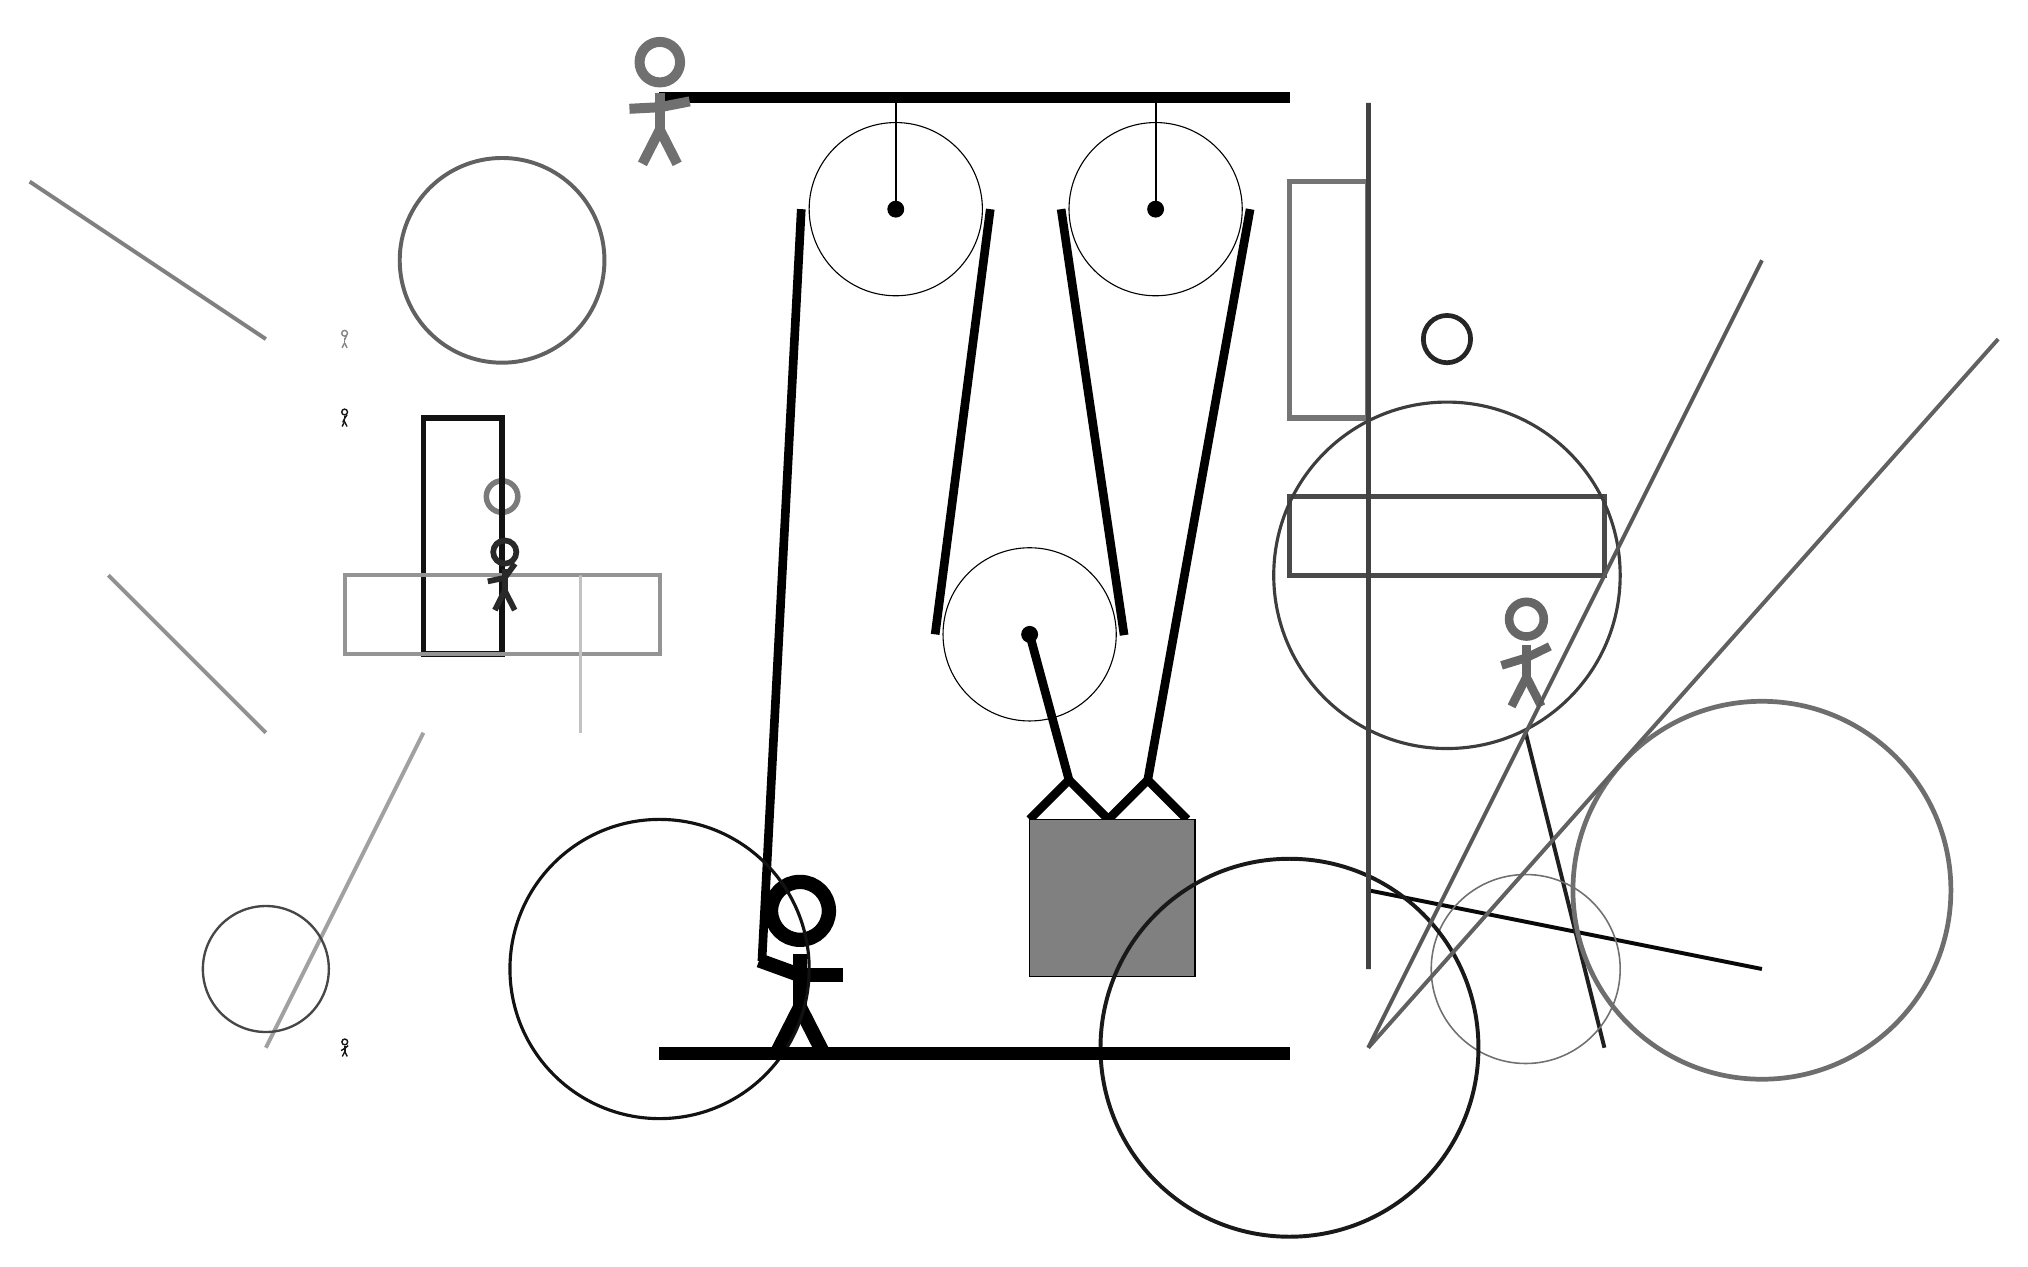
\begin{tikzpicture}
			%%%%% START %%%%%
			
			\draw[fill=black] (-2, 9) rectangle (6, 9.125);
			
			\draw (1, 7.65) circle (1.1);
			\draw[fill=black] (1, 7.65) circle (0.1);
			\draw[thick] (1, 7.65) -- (1, 9);
			
			\draw (4.3, 7.65) circle (1.1);
			\draw[fill=black] (4.3, 7.65) circle (0.1);
			\draw[thick] (4.3, 7.65) -- (4.3, 9);
			
			\draw (2.7, 2.25) circle (1.1);
			\draw[fill=black] (2.7, 2.25) circle (0.1);
			
			\draw[line width=1.1mm]  (2.7, -0.1) -- (3.2, 0.4) -- (3.7, -0.1) -- (4.2, 0.4) -- (4.7, -0.1);
			\draw[fill=black!50] (2.7, -0.1) rectangle (4.8, -2.1);
			
			\draw[line width=1.1mm](-0.7, -1.9) -- (-0.2, 7.65);
			\centerarc[line width=1.1mm](1, 7.65)(0:180:1.2000000000000002);
			\draw[line width=1.1mm](2.2, 7.65) -- (1.5, 2.25);
			\centerarc[line width=1.1mm](2.7, 2.25)(180:370:1.2000000000000002);
			\draw[line width=1.1mm] (3.9, 2.24) -- (3.1, 7.65);
			\centerarc[line width=1.1mm](4.3, 7.65)(0:180:1.2000000000000002);
			\draw[line width=1.1mm](4.2, 0.4) -- (5.5, 7.65);
			\draw[line width=1.1mm] (3.2, 0.4) -- (2.7, 2.25);
			
			\node at (-0.2, -2) {\Strichmaxerl[10][-20][0]};
			
			\draw [line width=0.6mm, color=black!85](8, 6) circle (0.3);
			
			\draw[line width=0.5mm, color=black!97](7, -1) -- (12, -2);
			\draw [line width=0.7mm, color=black!52](-4, 4) circle (0.2);
			\draw [line width=0.4mm, color=black!93](-2, -2) circle (1.9);
			
			\draw[line width=0.7mm, color=black!93] (-4, 2) rectangle (-5, 5);
			\draw[line width=0.5mm, color=black!88](9, 1) -- (10, -3);
			\draw[line width=0.5mm, color=black!42] (-2, 3) rectangle (-6, 2);
			\draw[line width=0.6mm, color=black!71] (6, 4) rectangle (10, 3);
			\draw [line width=0.6mm, color=black!57](12, -1) circle (2.4);
			\draw [line width=0.2mm, color=black!56](9, -2) circle (1.2);
			\draw[line width=0.5mm, color=black!50](-7, 6) -- (-10, 8);
			
			\node[line width=0.3mm, color=black!48] at (-6, 6) {\Strichmaxerl[1][90][64]};
			\draw[line width=0.5mm, color=black!37](-5, 1) -- (-7, -3);
			
			\draw [line width=0.5mm, color=black!90](6, -3) circle (2.4);
			\draw [line width=0.4mm, color=black!76](8, 3) circle (2.2);
			\node[line width=0.5mm, color=black!90] at (-6, 5) {\Strichmaxerl[1][65][56]};
			
			\draw[line width=0.7mm, color=black!54] (7, 8) rectangle (6, 5);
			\draw[line width=0.4mm, color=black!24] (-3, 1) rectangle (-3, 3);
			\draw [line width=0.5mm, color=black!62](-4, 7) circle (1.3);
			\draw[line width=0.5mm, color=black!62](7, -3) -- (15, 6);
			\node[line width=0.6mm, color=black!60] at (9, 2) {\Strichmaxerl[6][17][26]};
			\draw [line width=0.3mm, color=black!72](-7, -2) circle (0.8);
			
			\node[line width=0.5mm, color=black!91] at (-6, -3) {\Strichmaxerl[1][31][40]};
			\node[line width=0.6mm, color=black!84] at (-4, 3) {\Strichmaxerl[4][12][54]};
			\draw[line width=0.6mm, color=black!74] (7, 9) rectangle (7, -2);
			
			\draw[line width=0.5mm, color=black!43](-7, 1) -- (-9, 3);
			\node[line width=0.2mm, color=black!56] at (-2, 9) {\Strichmaxerl[7][3][11]};
			\draw[line width=0.5mm, color=black!65](7, -3) -- (12, 7);
			
			\draw[fill=black] (-2, -3) rectangle (6, -3.15);
			
			%%%%% END %%%%%
		\end{tikzpicture}
	\end{figure}	
\end{document}